\chapter{国际影响力}
\label{chapter:impact}
习近平总书记强调,科技创新是新质生产力的核心动力,尤其在全国两会等重大契机下更显重要。在“人工智能+”背景下,科技创新不仅推动国内经济发展,还显著提升“中国制造”的国际竞争力。通过教育改革、人才培养、生产方式变革、产业升级以及优化就业结构,科技创新为国家注入新动能,激发社会活力,使中国在全球科技竞争中占据关键地位。

\section{社会变革下的政府措施}
在全球科技迅猛发展的背景下,人工智能(AI)作为新一轮产业变革的核心驱动力,正逐步成为衡量一国科技竞争力与治理能力的重要指标。基于和鲸平台的调研数据,制作出“各地区AI相关透明度措施采用情况”面积图(见图\ref{各地区AI相关透明度措施采用情况图}),直观展示了不同区域在AI透明度措施上的采纳情况。
\begin{figure}[H]
    \centering
    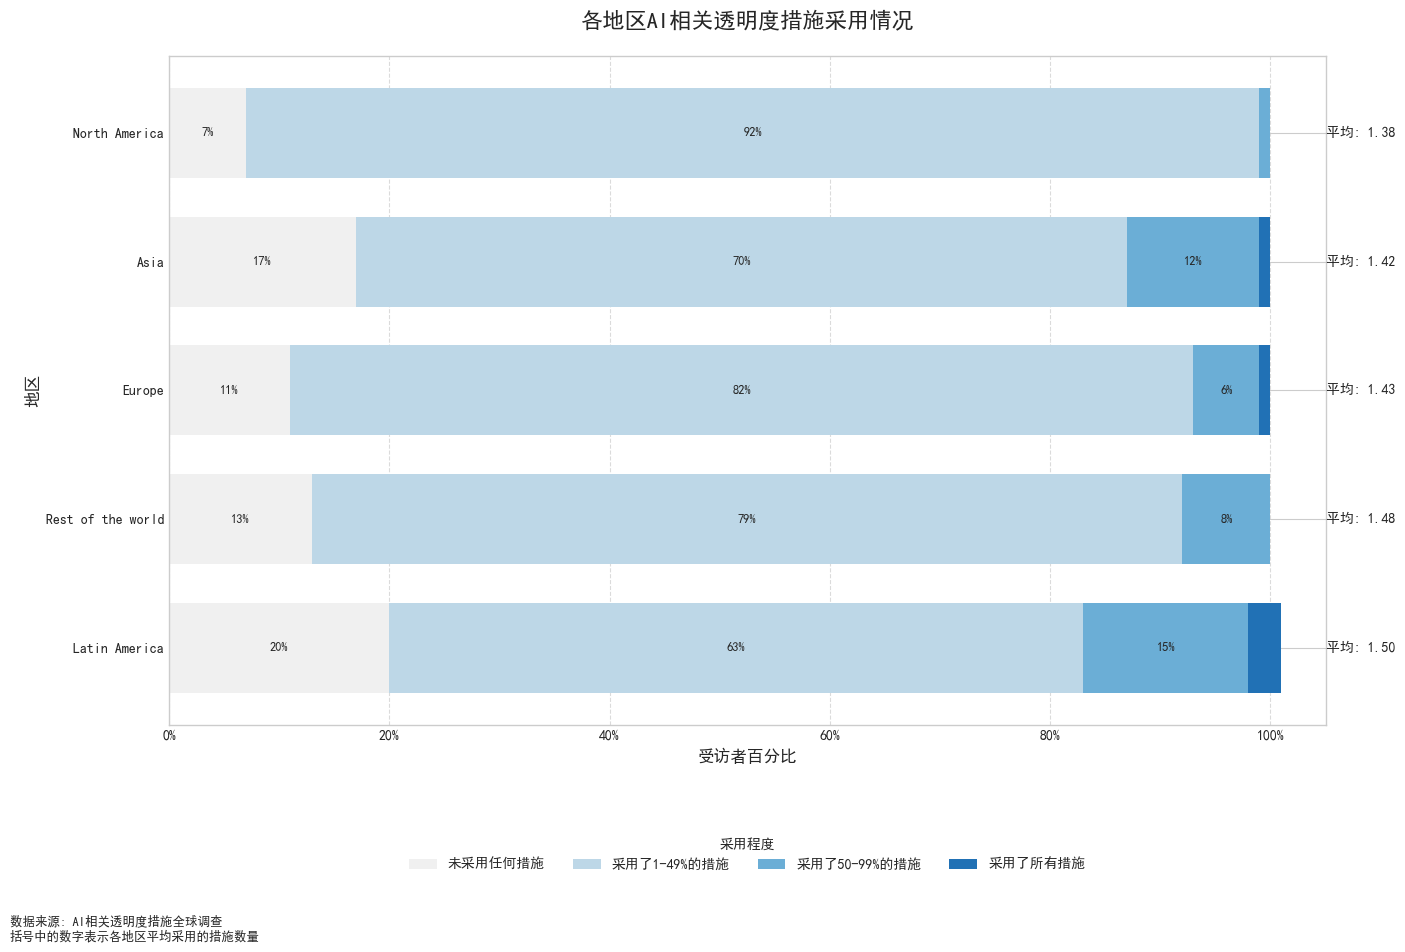
\includegraphics[width=0.7\linewidth]{figure/21各地区AI相关透明度措施采用情况图.png}
    \caption{各地区AI相关透明度措施采用情况图}
    \label{各地区AI相关透明度措施采用情况图}
\end{figure}

具体来看,北美在推广AI透明度政策上遥遥领先,高达92\%的机构已采用75\%至99\%的相关措施,另有7\%全面落实,显示出其治理框架的成熟。相比之下,亚洲70\%的机构仅执行中等级别(7\%至49\%)的措施,17\%的机构无任何行动,只有12\%的机构达到较高标准,反映出政策响应与技术实施的不均衡。欧洲则呈现两极分化:62\%的机构部分采纳,11\%的机构完全未响应,仅有6\%的机构实现全面落实,表明其制度虽具坚实基础,但执行深度仍不足。

总体而言,全球AI透明度措施推广虽已展开,但各区域在落实深度和广度上存在显著差异。北美政策体系完善但全面落实不足;亚洲与欧洲受国家发展和政策整合水平限制;而拉丁美洲及其他地区的迅速进展,则显示出新兴市场在数字治理中的潜力。

因此,我国在持续推出AI治理措施的同时,应注重提升政策执行的全面性与协调性,实现科技创新与社会责任的平衡,进而构建符合时代需求的AI治理新格局,稳步提升在全球科技生态中的话语权和引领力。\cite{butcher2023global}
\section{全球各国创新指数}
在全球科技迅猛发展的当下,创新已成为衡量一个国家综合国力与国际竞争力的关键指标。为了全面、系统地评估各国创新能力,世界知识产权组织每年发布《全球创新指数》,该指数整合了创新环境、投入、产出与成效等多个维度(见表\ref{创新指数构成表_上}和\ref{创新指数构成表_下}),已成为国际上广泛采用的重要评价工具。

根据国家统计局发布的创新指标构成数据(基准年份为2015年),以指数化形式展现各项指标的变化趋势(见图\ref{中国创新指数及分领域指数趋势图},旨在剖析我国近年来在创新领域取得的显著进步以及全球排名的稳步攀升。

\begin{figure}[H]
    \centering
    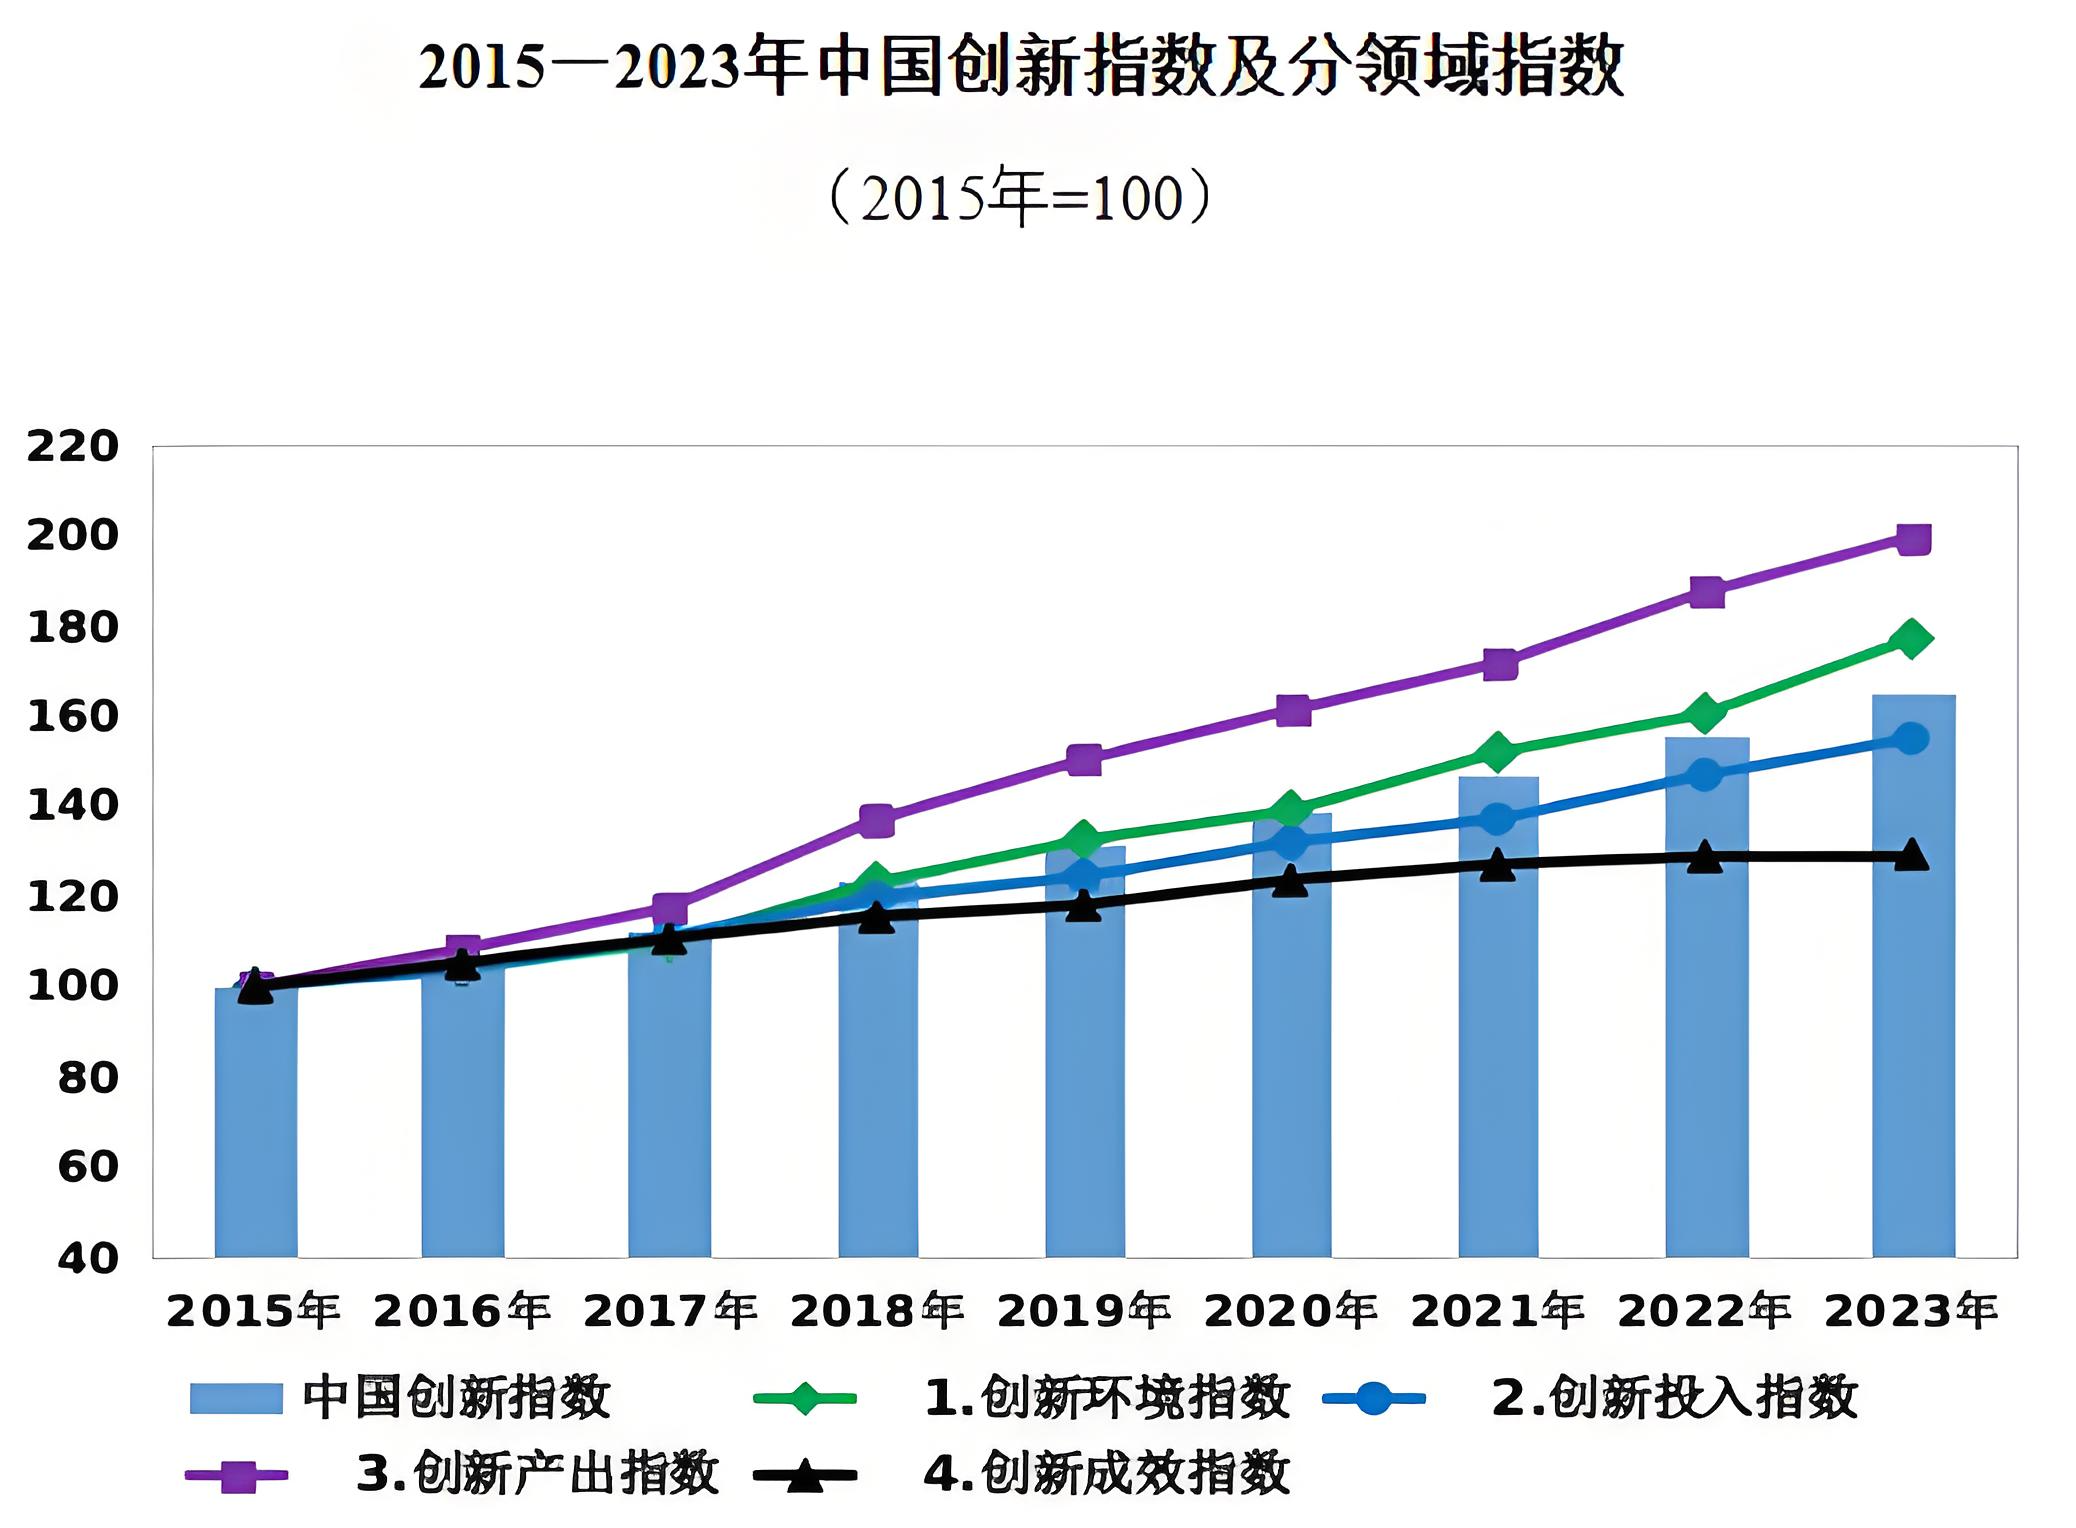
\includegraphics[width=0.7\linewidth]{figure/22中国创新指数及分领域指数趋势图.png}
    \caption{中国创新指数及分领域指数趋势图}
    \label{中国创新指数及分领域指数趋势图}
\end{figure}
自2015年设定基准(指数=100)以来,中国各项创新指标持续上扬,彰显结构优化与质量提升。总体创新指数至2023年接近180,显示出显著增长;其中,“创新产出指数”最为突出,从100迅速跃升至近210,反映科研成果显性化、技术转化效率提升及科技影响力增强;“创新投入指数”增长至近160,而“创新环境”和“创新成效指数”分别达约140与120,表明制度保障、科研氛围与教育支撑日趋完善。

尤其值得关注的是,中国在全球创新指数排名中实现历史性跃升。2024年数据显示,在132个评价国家中,中国位列第11,标志着从追赶者向引领者的转变,与长期位居前十的创新强国相比,凸显出国家科技战略的深远成效。

综上,通过量化分析及国际对比可见:中国在科技创新与自主研发能力提升上取得了实质性突破,国际竞争力显著增强。未来,若进一步深化科技体制改革、强化原始创新并推动成果转化,中国有望在更多关键领域实现从跟跑到并跑乃至领跑。建议后续补充高分辨率趋势图,以增强数据可视化和论文支撑。
\section{高技术产品出口比例}
在全球经济格局深度演变的背景下,高技术产品出口占制造业出口的比重已逐渐成为衡量一国技术发展水平和国际市场竞争力的重要指标。根据世界银行集团最新发布的数据,制作出“高技术产品出口占制造业出口的百分比”折线图(见图\ref{各国高技术产品出口占制造业出口比例趋势图}),直观展示了这一比重的变化趋势。

\begin{figure}[H]
    \centering
    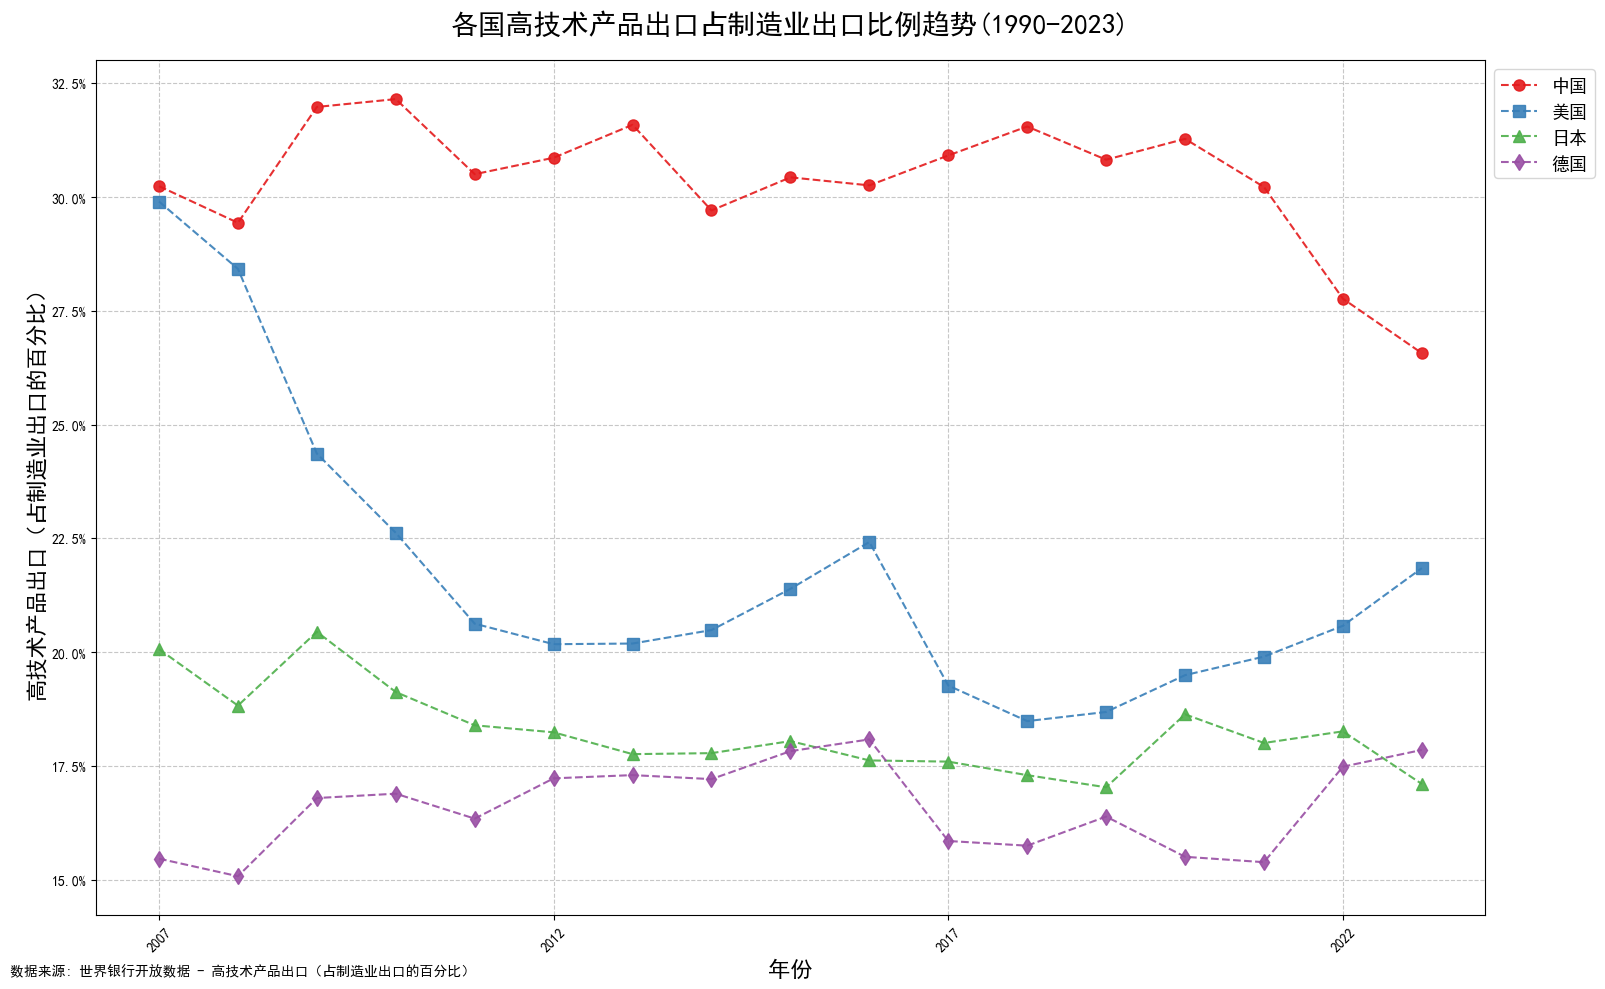
\includegraphics[width=0.7\linewidth]{figure/23各国高技术产品出口占制造业出口比例趋势图.png}
    \caption{各国高技术产品出口占制造业出口比例趋势图}
    \label{各国高技术产品出口占制造业出口比例趋势图}
\end{figure}

根据图示数据,自21世纪初以来,中国一直在该指标上保持领先,长期维持在约30\%的高位,远超美国、日本和德国。然而,自2021年以来,高技术产品出口比例明显下滑,截至2023年降至约27.5\%。同期,美国呈现温和回升,日本和德国则稳定在20\%及以下。这一变化引发了对我国高技术产业发展逻辑和外贸结构调整背景的关注,亟需多角度系统分析其内在驱动因素。

\textbf{(a) 全球竞争加剧}

近年来,越南、墨西哥及中东欧国家(如波兰、匈牙利)在全球制造业供应链中崛起,凭借低劳动力成本、优惠贸易政策与地理优势吸引大量投资。

\textbf{(b) 经济政策和产业结构调整}

近年来,中国经济政策逐步从出口导向转为内需和服务业驱动,同时推动制造业向高端和绿色转型,致使传统高技术产品在总出口中的比重下降。

\textbf{(c) 产能过剩和价格竞争}

部分高技术领域(如光伏、锂电池)存在产能过剩,导致国内竞争激烈、价格下跌,虽增强全球市场竞争力,却压缩了出口利润和比重。

\textbf{(d) 高技术产业分类和统计变化}

随着技术进步,高技术产品的定义和分类不断演变。新兴产业,如电动汽车和智能设备,可能未完全纳入传统统计范畴,导致高技术出口比重下降。

综上所述,中国高技术产品出口占比的下降,并不意味着技术能力衰退,而是多重因素作用的结果。\cite{li2021china}未来,政策制定者应结合全球市场动态优化出口结构,并通过技术创新和制度升级提升产品附加值及议价能力,从而巩固并扩大中国在全球高技术领域的战略优势。
\section{新产品投入产出}
为了全面剖析我国高技术产品出口结构的演化趋势及背后驱动逻辑,本节以“新产品投入产出”为切入点,构建“传统高技术产业出口下滑—新兴产业快速兴起—创新结构转型升级”的因果链,揭示中国在全球技术竞争中的战略调整。

基于国家统计局与和鲸平台提供的《规模以上工业企业的科技活动基本情况》数据集,绘制出2004至2023年工业企业“新产品投入产出比”柱状图(见图\ref{工业企业新产品投入产出对比}),聚焦“新三样”产业(电动载人汽车、锂离子蓄电池、太阳能电池)的迅速发展,为理解高技术出口占比下降背后的转型逻辑提供了坚实数据支撑。

\begin{figure}[H]
    \centering
    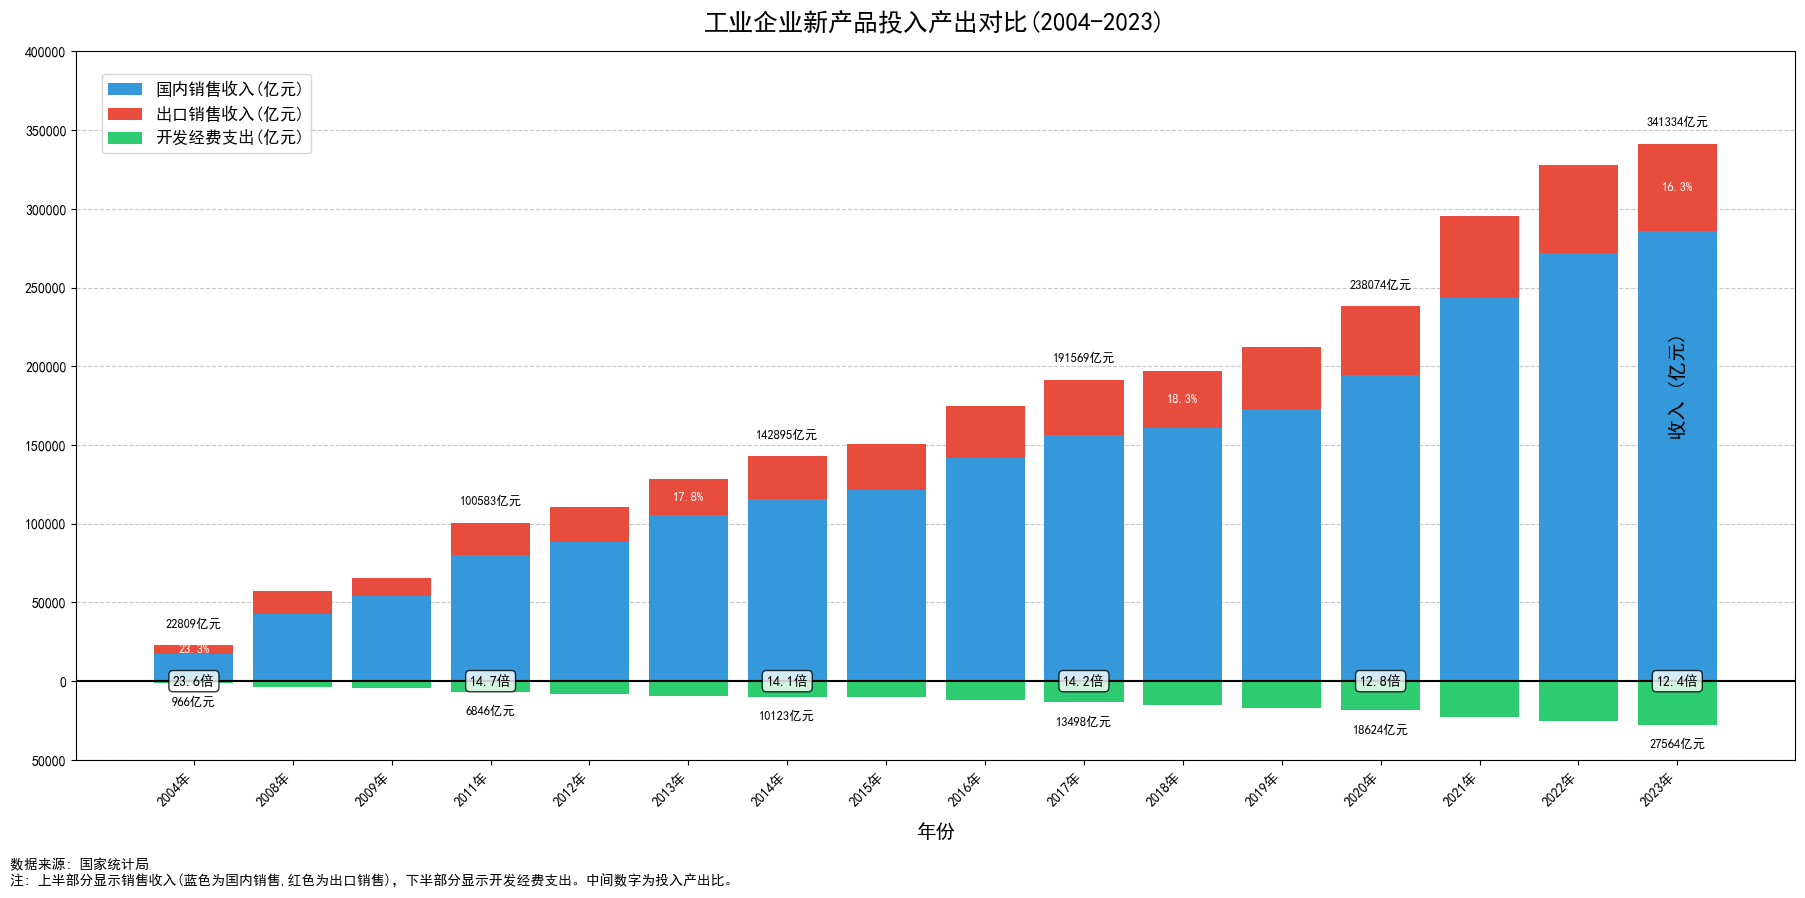
\includegraphics[width=0.7\linewidth]{figure/24工业企业新产品投入产出对比.png}
    \caption{工业企业新产品投入产出对比图}
    \label{工业企业新产品投入产出对比}
\end{figure}

自2011年以来,新产品销售收入从不足1.1万亿元飙升至2023年的34.1万亿元,增幅超30倍,年均复合增长率达20\%以上;其中出口销售收入从2015年的13.5万亿元增至2023年的27.5万亿元,接近翻倍。这表明,即便传统统计中高技术产品出口占比下降,其绝对出口额正大幅提高,中国正在从传统高技术向新兴高技术转型。

同时,2011至2023年间,研发投入与销售额的比值稳定在约12~14倍,显示新兴产业研发产出效率高、成果转化能力强。尤其2020年后,“新基建”与绿色能源政策推动电动汽车、储能电池和光伏组件等产业爆发式增长,2023年其出口增幅分别达67\%、32\%和30.5\%,虽未完全涵盖传统高技术统计,但技术含量和附加值已符合甚至超越高技术标准。

此外,工业企业研发投入于2023年达到2.8万亿元,占新产品销售额的8\%以上,形成了良性研发—产出循环,提升了产业链附加值与全球竞争力,如宁德时代、比亚迪和隆基绿能等企业在出口上持续扩大领先优势。

总体来说,高技术产品出口占比下降的背后,隐藏着新兴技术产业的崛起和结构升级,标志着中国正由传统出口向创新驱动型出口转型。\cite{zhou2021technological}